\chapter{Animation}
\begin{figure}[htb]
    \centering
    \begin{subfigure}[b]{0.6\textwidth}
        \centering
        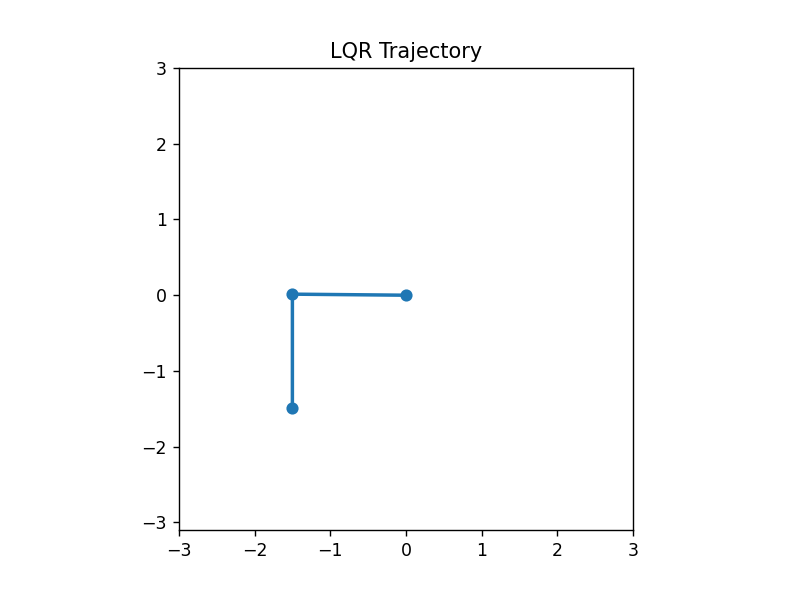
\includegraphics[width=\linewidth]{img/Animation/Eq1.png}
        \caption{Equilibrium point 1}
        \label{fig:eq1}
    \end{subfigure}
    \hfill
    \begin{subfigure}[b]{0.6\textwidth}
        \centering
        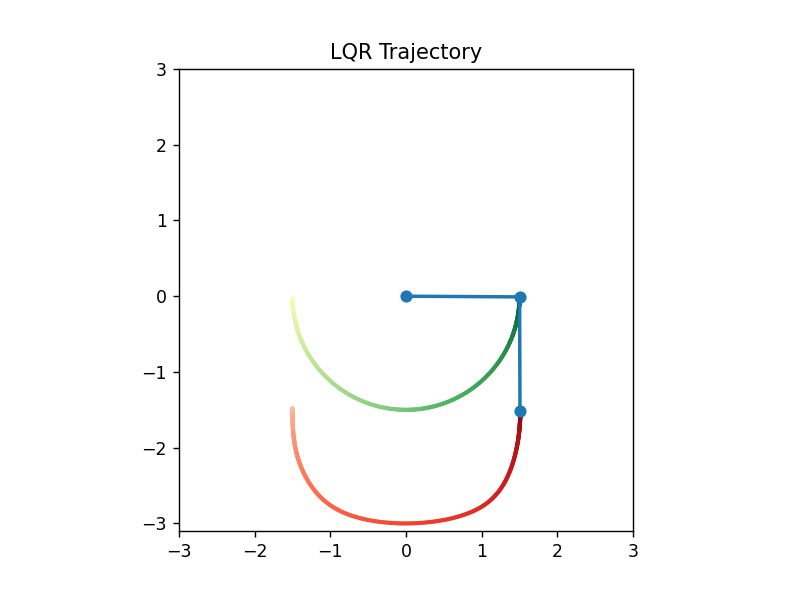
\includegraphics[width=\linewidth]{img/Animation/Eq2.png}
        \caption{Equilibrium point 2}
        \label{fig:eq2}
    \end{subfigure}
    \caption{}
    \label{fig:equilibrium-set1}
\end{figure}

\begin{figure}[htb]
    \centering
    \begin{subfigure}[b]{0.7\textwidth}
        \centering
        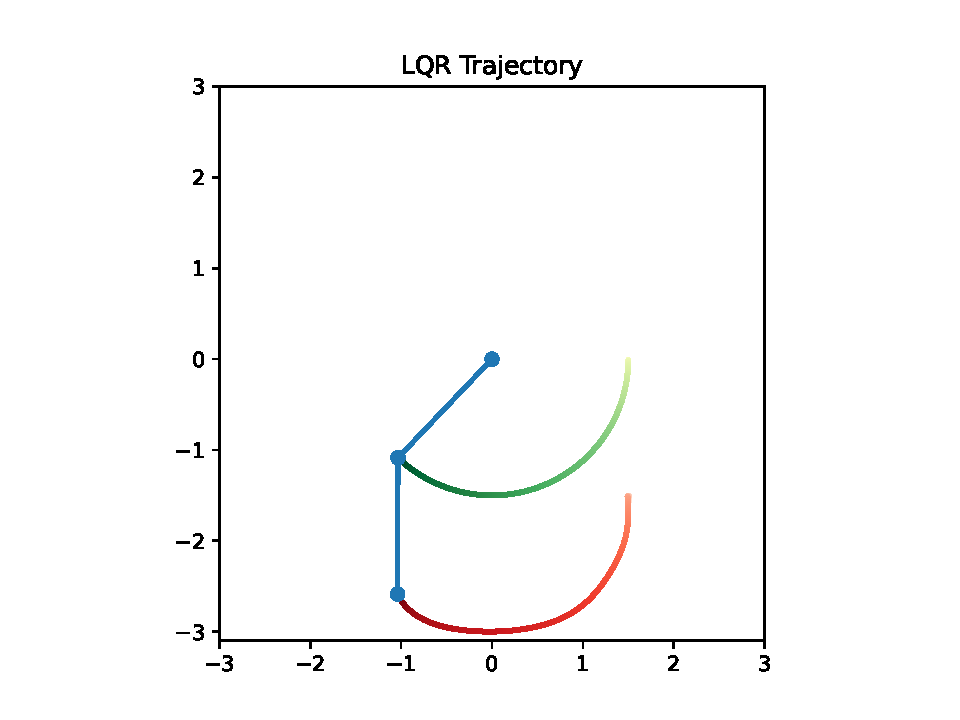
\includegraphics[width=\linewidth]{img/Animation/Eq3.pdf}
        \caption{Equilibrium point 3}
        \label{fig:eq3}
    \end{subfigure}
    \hfill
    \begin{subfigure}[b]{0.7\textwidth}
        \centering
        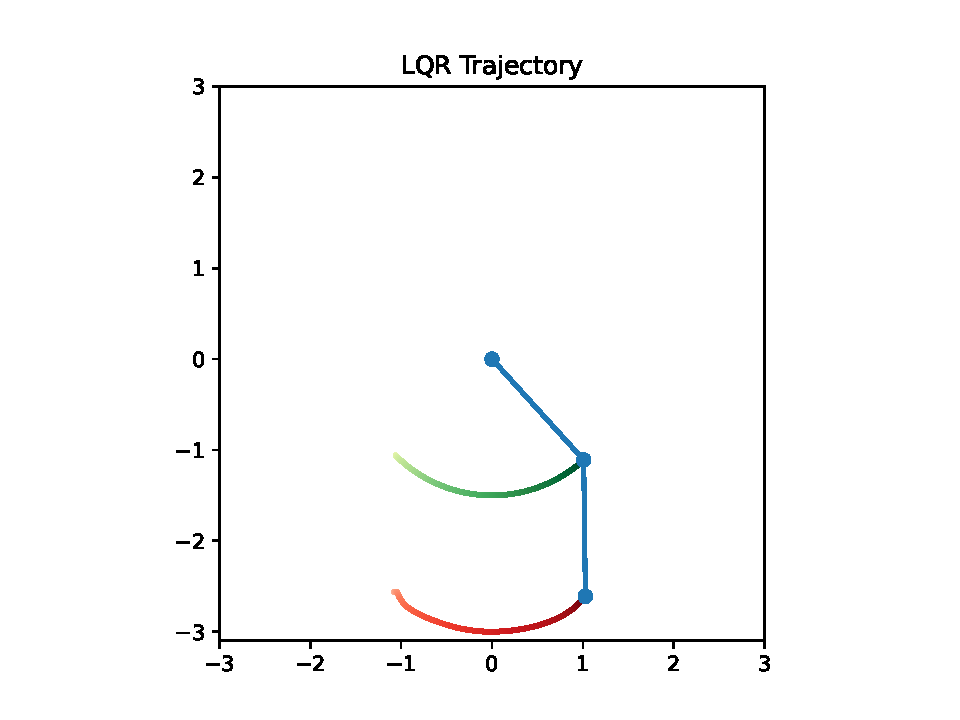
\includegraphics[width=\linewidth]{img/Animation/Eq4.pdf}
        \caption{Equilibrium point 4}
        \label{fig:eq4}
    \end{subfigure}
    
    \vspace{1em}
    
    \begin{subfigure}[b]{0.7\textwidth}
        \centering
        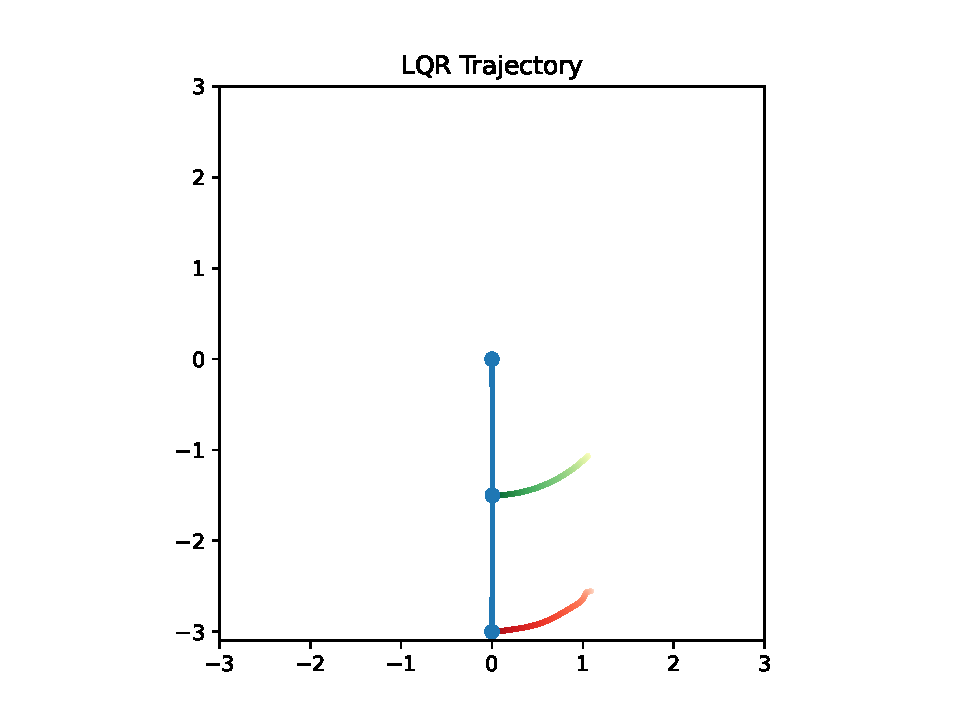
\includegraphics[width=\linewidth]{img/Animation/Eq5.pdf}
        \caption{Equilibrium point 5}
        \label{fig:eq5}
    \end{subfigure}
    \caption{}
    \label{fig:equilibrium-set2}
\end{figure}


% - Describe tools and methodology for creating the animation Python
% - Highlight what the animation demonstrates (e.g., robot motion for Task 3).

\chapter*{Conclusions}
% - Summarize findings from the project.
% - Discuss the effectiveness of the methods used.
% - Mention limitations and propose future work directions.

This work addresses the optimal control of a planar underactuated two-link robotic manipulator. The system dynamics were discretized, and the system's evolution was observed to be consistent and promising. Newton's method for root finding, used to compute the equilibria, proved to be highly effective. Also the reference generation for a quasi-static trajectory also demonstrated strong performance. Additionally, the formulation of a quadratic cost function effectively penalized errors in both states and inputs.

In Task 1, although significant results were achieved, the Armijo plots were sometimes not representative in the last iterations of the algorithm. Several potential causes could explain this issue. One possibility is numerical instability, which can occur when handling extremely large or small values and the precision is crucial. The use of a step reference may exacerbate this problem due to its lack of continuity.

In Task 2 a smooth reference curve was employed. In this case, the Armijo plots appeared accurate, with the descent direction consistently tangent to the cost function. Furthermore, the plot's scale indicated that the cost function's slope decreased over time, resulting in the Armijo method taking more steps as expected when nearing convergence.

The trajectory tracking task using Linear Quadratic Regulator (LQR) control was successfully implemented to design an optimal feedback control. The results demonstrated that the controller could rapidly eliminate disturbances applied at the initial condition. Since the inputs were not constrained, the control was highly aggressive initially, quickly removing oscillations. However, when disturbances increased, some oscillations were not entirely eliminated.

Trajectory tracking using Model Predictive Control (MPC) demonstrated robustness to both state and input perturbations. In cases 1 and 2, the same disturbance values were applied at the initial condition as in cases 2 and 3 of the LQR. A comparison revealed that LQR quickly mitigated perturbations but struggled with larger disturbances. In contrast, MPC effectively compensated for even larger disturbances, as observed in case 3. Additionally, MPC managed Gaussian noise in both sensor readings and actuation effectively while adhering to constraints on input and state variations. However, as noise levels increased, noticeable oscillations in actuation arose, a result of the controller's aggressive behavior. These oscillations could potentially be mitigated by imposing constraints on input variation over time. Another drawback of the MPC was the limited prediction window. While this constraint enables real-time applications, it reduces the controller's overall effectiveness.

The animations provided demonstrated satisfactory results across all tasks, as the references were closely followed and oscillations were eliminated through actuation.